
%% bare_jrnl.tex
%% V1.4
%% 2012/12/27
%% by Michael Shell
%% see http://www.michaelshell.org/
%% for current contact information.
%%
%% This is a skeleton file demonstrating the use of IEEEtran.cls
%% (requires IEEEtran.cls version 1.8 or later) with an IEEE journal paper.
%%
%% Support sites:
%% http://www.michaelshell.org/tex/ieeetran/
%% http://www.ctan.org/tex-archive/macros/latex/contrib/IEEEtran/
%% and
%% http://www.ieee.org/



% *** Authors should verify (and, if needed, correct) their LaTeX system  ***
% *** with the testflow diagnostic prior to trusting their LaTeX platform ***
% *** with production work. IEEE's font choices can trigger bugs that do  ***
% *** not appear when using other class files.                            ***
% The testflow support page is at:
% http://www.michaelshell.org/tex/testflow/


%%*************************************************************************
%% Legal Notice:
%% This code is offered as-is without any warranty either expressed or
%% implied; without even the implied warranty of MERCHANTABILITY or
%% FITNESS FOR A PARTICULAR PURPOSE! 
%% User assumes all risk.
%% In no event shall IEEE or any contributor to this code be liable for
%% any damages or losses, including, but not limited to, incidental,
%% consequential, or any other damages, resulting from the use or misuse
%% of any information contained here.
%%
%% All comments are the opinions of their respective authors and are not
%% necessarily endorsed by the IEEE.
%%
%% This work is distributed under the LaTeX Project Public License (LPPL)
%% ( http://www.latex-project.org/ ) version 1.3, and may be freely used,
%% distributed and modified. A copy of the LPPL, version 1.3, is included
%% in the base LaTeX documentation of all distributions of LaTeX released
%% 2003/12/01 or later.
%% Retain all contribution notices and credits.
%% ** Modified files should be clearly indicated as such, including  **
%% ** renaming them and changing author support contact information. **
%%
%% File list of work: IEEEtran.cls, IEEEtran_HOWTO.pdf, bare_adv.tex,
%%                    bare_conf.tex, bare_jrnl.tex, bare_jrnl_compsoc.tex,
%%                    bare_jrnl_transmag.tex
%%*************************************************************************

% Note that the a4paper option is mainly intended so that authors in
% countries using A4 can easily print to A4 and see how their papers will
% look in print - the typesetting of the document will not typically be
% affected with changes in paper size (but the bottom and side margins will).
% Use the testflow package mentioned above to verify correct handling of
% both paper sizes by the user's LaTeX system.
%
% Also note that the "draftcls" or "draftclsnofoot", not "draft", option
% should be used if it is desired that the figures are to be displayed in
% draft mode.
%
\documentclass[journal]{IEEEtran}
%
% If IEEEtran.cls has not been installed into the LaTeX system files,
% manually specify the path to it like:
% \documentclass[journal]{../sty/IEEEtran}





% Some very useful LaTeX packages include:
% (uncomment the ones you want to load)


% *** MISC UTILITY PACKAGES ***
%
%\usepackage{ifpdf}
% Heiko Oberdiek's ifpdf.sty is very useful if you need conditional
% compilation based on whether the output is pdf or dvi.
% usage:
% \ifpdf
%   % pdf code
% \else
%   % dvi code
% \fi
% The latest version of ifpdf.sty can be obtained from:
% http://www.ctan.org/tex-archive/macros/latex/contrib/oberdiek/
% Also, note that IEEEtran.cls V1.7 and later provides a builtin
% \ifCLASSINFOpdf conditional that works the same way.
% When switching from latex to pdflatex and vice-versa, the compiler may
% have to be run twice to clear warning/error messages.






% *** CITATION PACKAGES ***
%
%\usepackage{cite}
% cite.sty was written by Donald Arseneau
% V1.6 and later of IEEEtran pre-defines the format of the cite.sty package
% \cite{} output to follow that of IEEE. Loading the cite package will
% result in citation numbers being automatically sorted and properly
% "compressed/ranged". e.g., [1], [9], [2], [7], [5], [6] without using
% cite.sty will become [1], [2], [5]--[7], [9] using cite.sty. cite.sty's
% \cite will automatically add leading space, if needed. Use cite.sty's
% noadjust option (cite.sty V3.8 and later) if you want to turn this off
% such as if a citation ever needs to be enclosed in parenthesis.
% cite.sty is already installed on most LaTeX systems. Be sure and use
% version 4.0 (2003-05-27) and later if using hyperref.sty. cite.sty does
% not currently provide for hyperlinked citations.
% The latest version can be obtained at:
% http://www.ctan.org/tex-archive/macros/latex/contrib/cite/
% The documentation is contained in the cite.sty file itself.






% *** GRAPHICS RELATED PACKAGES ***
%
\ifCLASSINFOpdf
   \usepackage[pdftex]{graphicx}
   \graphicspath{{../pdf/}{../jpeg/}}
  % and their extensions so you won't have to specify these with
  % every instance of \includegraphics
   \DeclareGraphicsExtensions{.pdf,.jpeg,.png}
\else
  % or other class option (dvipsone, dvipdf, if not using dvips). graphicx
  % will default to the driver specified in the system graphics.cfg if no
  % driver is specified.
   \usepackage[dvips]{graphicx}
  % declare the path(s) where your graphic files are
   \graphicspath{{../eps/}}
  % and their extensions so you won't have to specify these with
  % every instance of \includegraphics
   \DeclareGraphicsExtensions{.eps}
\fi
% graphicx was written by David Carlisle and Sebastian Rahtz. It is
% required if you want graphics, photos, etc. graphicx.sty is already
% installed on most LaTeX systems. The latest version and documentation
% can be obtained at: 
% http://www.ctan.org/tex-archive/macros/latex/required/graphics/
% Another good source of documentation is "Using Imported Graphics in
% LaTeX2e" by Keith Reckdahl which can be found at:
% http://www.ctan.org/tex-archive/info/epslatex/
%
% latex, and pdflatex in dvi mode, support graphics in encapsulated
% postscript (.eps) format. pdflatex in pdf mode supports graphics
% in .pdf, .jpeg, .png and .mps (metapost) formats. Users should ensure
% that all non-photo figures use a vector format (.eps, .pdf, .mps) and
% not a bitmapped formats (.jpeg, .png). IEEE frowns on bitmapped formats
% which can result in "jaggedy"/blurry rendering of lines and letters as
% well as large increases in file sizes.
%
% You can find documentation about the pdfTeX application at:
% http://www.tug.org/applications/pdftex





% *** MATH PACKAGES ***
%
%\usepackage[cmex10]{amsmath}
% A popular package from the American Mathematical Society that provides
% many useful and powerful commands for dealing with mathematics. If using
% it, be sure to load this package with the cmex10 option to ensure that
% only type 1 fonts will utilized at all point sizes. Without this option,
% it is possible that some math symbols, particularly those within
% footnotes, will be rendered in bitmap form which will result in a
% document that can not be IEEE Xplore compliant!
%
% Also, note that the amsmath package sets \interdisplaylinepenalty to 10000
% thus preventing page breaks from occurring within multiline equations. Use:
%\interdisplaylinepenalty=2500
% after loading amsmath to restore such page breaks as IEEEtran.cls normally
% does. amsmath.sty is already installed on most LaTeX systems. The latest
% version and documentation can be obtained at:
% http://www.ctan.org/tex-archive/macros/latex/required/amslatex/math/





% *** SPECIALIZED LIST PACKAGES ***
%
%\usepackage{algorithmic}
% algorithmic.sty was written by Peter Williams and Rogerio Brito.
% This package provides an algorithmic environment fo describing algorithms.
% You can use the algorithmic environment in-text or within a figure
% environment to provide for a floating algorithm. Do NOT use the algorithm
% floating environment provided by algorithm.sty (by the same authors) or
% algorithm2e.sty (by Christophe Fiorio) as IEEE does not use dedicated
% algorithm float types and packages that provide these will not provide
% correct IEEE style captions. The latest version and documentation of
% algorithmic.sty can be obtained at:
% http://www.ctan.org/tex-archive/macros/latex/contrib/algorithms/
% There is also a support site at:
% http://algorithms.berlios.de/index.html
% Also of interest may be the (relatively newer and more customizable)
% algorithmicx.sty package by Szasz Janos:
% http://www.ctan.org/tex-archive/macros/latex/contrib/algorithmicx/




% *** ALIGNMENT PACKAGES ***
%
%\usepackage{array}
% Frank Mittelbach's and David Carlisle's array.sty patches and improves
% the standard LaTeX2e array and tabular environments to provide better
% appearance and additional user controls. As the default LaTeX2e table
% generation code is lacking to the point of almost being broken with
% respect to the quality of the end results, all users are strongly
% advised to use an enhanced (at the very least that provided by array.sty)
% set of table tools. array.sty is already installed on most systems. The
% latest version and documentation can be obtained at:
% http://www.ctan.org/tex-archive/macros/latex/required/tools/


% IEEEtran contains the IEEEeqnarray family of commands that can be used to
% generate multiline equations as well as matrices, tables, etc., of high
% quality.




% *** SUBFIGURE PACKAGES ***
%\ifCLASSOPTIONcompsoc
%  \usepackage[caption=false,font=normalsize,labelfont=sf,textfont=sf]{subfig}
%\else
%  \usepackage[caption=false,font=footnotesize]{subfig}
%\fi
% subfig.sty, written by Steven Douglas Cochran, is the modern replacement
% for subfigure.sty, the latter of which is no longer maintained and is
% incompatible with some LaTeX packages including fixltx2e. However,
% subfig.sty requires and automatically loads Axel Sommerfeldt's caption.sty
% which will override IEEEtran.cls' handling of captions and this will result
% in non-IEEE style figure/table captions. To prevent this problem, be sure
% and invoke subfig.sty's "caption=false" package option (available since
% subfig.sty version 1.3, 2005/06/28) as this is will preserve IEEEtran.cls
% handling of captions.
% Note that the Computer Society format requires a larger sans serif font
% than the serif footnote size font used in traditional IEEE formatting
% and thus the need to invoke different subfig.sty package options depending
% on whether compsoc mode has been enabled.
%
% The latest version and documentation of subfig.sty can be obtained at:
% http://www.ctan.org/tex-archive/macros/latex/contrib/subfig/




% *** FLOAT PACKAGES ***
%
%\usepackage{fixltx2e}
% fixltx2e, the successor to the earlier fix2col.sty, was written by
% Frank Mittelbach and David Carlisle. This package corrects a few problems
% in the LaTeX2e kernel, the most notable of which is that in current
% LaTeX2e releases, the ordering of single and double column floats is not
% guaranteed to be preserved. Thus, an unpatched LaTeX2e can allow a
% single column figure to be placed prior to an earlier double column
% figure. The latest version and documentation can be found at:
% http://www.ctan.org/tex-archive/macros/latex/base/


%\usepackage{stfloats}
% stfloats.sty was written by Sigitas Tolusis. This package gives LaTeX2e
% the ability to do double column floats at the bottom of the page as well
% as the top. (e.g., "\begin{figure*}[!b]" is not normally possible in
% LaTeX2e). It also provides a command:
%\fnbelowfloat
% to enable the placement of footnotes below bottom floats (the standard
% LaTeX2e kernel puts them above bottom floats). This is an invasive package
% which rewrites many portions of the LaTeX2e float routines. It may not work
% with other packages that modify the LaTeX2e float routines. The latest
% version and documentation can be obtained at:
% http://www.ctan.org/tex-archive/macros/latex/contrib/sttools/
% Do not use the stfloats baselinefloat ability as IEEE does not allow
% \baselineskip to stretch. Authors submitting work to the IEEE should note
% that IEEE rarely uses double column equations and that authors should try
% to avoid such use. Do not be tempted to use the cuted.sty or midfloat.sty
% packages (also by Sigitas Tolusis) as IEEE does not format its papers in
% such ways.
% Do not attempt to use stfloats with fixltx2e as they are incompatible.
% Instead, use Morten Hogholm'a dblfloatfix which combines the features
% of both fixltx2e and stfloats:
%
% \usepackage{dblfloatfix}
% The latest version can be found at:
% http://www.ctan.org/tex-archive/macros/latex/contrib/dblfloatfix/




%\ifCLASSOPTIONcaptionsoff
%  \usepackage[nomarkers]{endfloat}
% \let\MYoriglatexcaption\caption
% \renewcommand{\caption}[2][\relax]{\MYoriglatexcaption[#2]{#2}}
%\fi
% endfloat.sty was written by James Darrell McCauley, Jeff Goldberg and 
% Axel Sommerfeldt. This package may be useful when used in conjunction with 
% IEEEtran.cls'  captionsoff option. Some IEEE journals/societies require that
% submissions have lists of figures/tables at the end of the paper and that
% figures/tables without any captions are placed on a page by themselves at
% the end of the document. If needed, the draftcls IEEEtran class option or
% \CLASSINPUTbaselinestretch interface can be used to increase the line
% spacing as well. Be sure and use the nomarkers option of endfloat to
% prevent endfloat from "marking" where the figures would have been placed
% in the text. The two hack lines of code above are a slight modification of
% that suggested by in the endfloat docs (section 8.4.1) to ensure that
% the full captions always appear in the list of figures/tables - even if
% the user used the short optional argument of \caption[]{}.
% IEEE papers do not typically make use of \caption[]'s optional argument,
% so this should not be an issue. A similar trick can be used to disable
% captions of packages such as subfig.sty that lack options to turn off
% the subcaptions:
% For subfig.sty:
% \let\MYorigsubfloat\subfloat
% \renewcommand{\subfloat}[2][\relax]{\MYorigsubfloat[]{#2}}
% However, the above trick will not work if both optional arguments of
% the \subfloat command are used. Furthermore, there needs to be a
% description of each subfigure *somewhere* and endfloat does not add
% subfigure captions to its list of figures. Thus, the best approach is to
% avoid the use of subfigure captions (many IEEE journals avoid them anyway)
% and instead reference/explain all the subfigures within the main caption.
% The latest version of endfloat.sty and its documentation can obtained at:
% http://www.ctan.org/tex-archive/macros/latex/contrib/endfloat/
%
% The IEEEtran \ifCLASSOPTIONcaptionsoff conditional can also be used
% later in the document, say, to conditionally put the References on a 
% page by themselves.




% *** PDF, URL AND HYPERLINK PACKAGES ***
%
%\usepackage{url}
% url.sty was written by Donald Arseneau. It provides better support for
% handling and breaking URLs. url.sty is already installed on most LaTeX
% systems. The latest version and documentation can be obtained at:
% http://www.ctan.org/tex-archive/macros/latex/contrib/url/
% Basically, \url{my_url_here}.




% *** Do not adjust lengths that control margins, column widths, etc. ***
% *** Do not use packages that alter fonts (such as pslatex).         ***
% There should be no need to do such things with IEEEtran.cls V1.6 and later.
% (Unless specifically asked to do so by the journal or conference you plan
% to submit to, of course. )


% correct bad hyphenation here
\hyphenation{op-tical net-works semi-conduc-tor}


\begin{document}
%
% paper title
% can use linebreaks \\ within to get better formatting as desired
% Do not put math or special symbols in the title.
\title{Passive device-free indoor localisation based on RSSI on a mobile phone}
%
%
% author names and IEEE memberships
% note positions of commas and nonbreaking spaces ( ~ ) LaTeX will not break
% a structure at a ~ so this keeps an author's name from being broken across
% two lines.
% use \thanks{} to gain access to the first footnote area
% a separate \thanks must be used for each paragraph as LaTeX2e's \thanks
% was not built to handle multiple paragraphs
%

% \author{Markus~Matoni,
%         Michael~Krawez,
%         Gipsa~Joseph
%         and~Stephan~Sigg% <-this % stops a space
% \thanks{M. Matoni, M. Shell and G. Joseph are with Goettingen University.}% <-this % stops a space
% \thanks{S. Sigg is with the networking group of Goettingen University, Germany}% <-this % stops a space
% }

\author{
}
% note the % following the last \IEEEmembership and also \thanks - 
% these prevent an unwanted space from occurring between the last author name
% and the end of the author line. i.e., if you had this:
% 
% \author{....lastname \thanks{...} \thanks{...} }
%                     ^------------^------------^----Do not want these spaces!
%
% a space would be appended to the last name and could cause every name on that
% line to be shifted left slightly. This is one of those "LaTeX things". For
% instance, "\textbf{A} \textbf{B}" will typeset as "A B" not "AB". To get
% "AB" then you have to do: "\textbf{A}\textbf{B}"
% \thanks is no different in this regard, so shield the last } of each \thanks
% that ends a line with a % and do not let a space in before the next \thanks.
% Spaces after \IEEEmembership other than the last one are OK (and needed) as
% you are supposed to have spaces between the names. For what it is worth,
% this is a minor point as most people would not even notice if the said evil
% space somehow managed to creep in.



% The paper headers
\markboth{Submitted to IPSN 2014 -- Indoor localization Competition}%
{Matoni \MakeLowercase{\textit{et al.}}: Demo of RSSI-based passive indoor localisation}
% The only time the second header will appear is for the odd numbered pages
% after the title page when using the twoside option.
% 
% *** Note that you probably will NOT want to include the author's ***
% *** name in the headers of peer review papers.                   ***
% You can use \ifCLASSOPTIONpeerreview for conditional compilation here if
% you desire.




% If you want to put a publisher's ID mark on the page you can do it like
% this:
%\IEEEpubid{0000--0000/00\$00.00~\copyright~2012 IEEE}
% Remember, if you use this you must call \IEEEpubidadjcol in the second
% column for its text to clear the IEEEpubid mark.



% use for special paper notices
%\IEEEspecialpapernotice{(Invited Paper)}




% make the title area
\maketitle

% As a general rule, do not put math, special symbols or citations
% in the abstract or keywords.
\begin{abstract}
We propose a device-free passive indoor localisation system by analysing the fluctuation in received RSSI packets received from environmental WiFi access points.
With a single device in each room the system is able to detect presence and to provide a broad classification of the actual location of a single person dividing the room into a grid of four regions. 
\end{abstract}

% Note that keywords are not normally used for peerreview papers.


% For peer review papers, you can put extra information on the cover
% page as needed:
% \ifCLASSOPTIONpeerreview
% \begin{center} \bfseries EDICS Category: 3-BBND \end{center}
% \fi
%
% For peerreview papers, this IEEEtran command inserts a page break and
% creates the second title. It will be ignored for other modes.
\IEEEpeerreviewmaketitle


% The very first letter is a 2 line initial drop letter followed
% by the rest of the first word in caps.
% 
% form to use if the first word consists of a single letter:
% \IEEEPARstart{A}{demo} file is ....
% 
% form to use if you need the single drop letter followed by
% normal text (unknown if ever used by IEEE):
% \IEEEPARstart{A}{}demo file is ....
% 
% Some journals put the first two words in caps:
% \IEEEPARstart{T}{his demo} file is ....
% 
% Here we have the typical use of a "T" for an initial drop letter
% and "HIS" in caps to complete the first word.




% needed in second column of first page if using \IEEEpubid
%\IEEEpubidadjcol




% An example of a floating figure using the graphicx package.
% Note that \label must occur AFTER (or within) \caption.
% For figures, \caption should occur after the \includegraphics.
% Note that IEEEtran v1.7 and later has special internal code that
% is designed to preserve the operation of \label within \caption
% even when the captionsoff option is in effect. However, because
% of issues like this, it may be the safest practice to put all your
% \label just after \caption rather than within \caption{}.
%
% Reminder: the "draftcls" or "draftclsnofoot", not "draft", class
% option should be used if it is desired that the figures are to be
% displayed while in draft mode.
%
%\begin{figure}[!t]
%\centering
%\includegraphics[width=2.5in]{myfigure}
% where an .eps filename suffix will be assumed under latex, 
% and a .pdf suffix will be assumed for pdflatex; or what has been declared
% via \DeclareGraphicsExtensions.
%\caption{Simulation Results.}
%\label{fig_sim}
%\end{figure}

% Note that IEEE typically puts floats only at the top, even when this
% results in a large percentage of a column being occupied by floats.


% An example of a double column floating figure using two subfigures.
% (The subfig.sty package must be loaded for this to work.)
% The subfigure \label commands are set within each subfloat command,
% and the \label for the overall figure must come after \caption.
% \hfil is used as a separator to get equal spacing.
% Watch out that the combined width of all the subfigures on a 
% line do not exceed the text width or a line break will occur.
%
%\begin{figure*}[!t]
%\centering
%\subfloat[Case I]{\includegraphics[width=2.5in]{box}%
%\label{fig_first_case}}
%\hfil
%\subfloat[Case II]{\includegraphics[width=2.5in]{box}%
%\label{fig_second_case}}
%\caption{Simulation results.}
%\label{fig_sim}
%\end{figure*}
%
% Note that often IEEE papers with subfigures do not employ subfigure
% captions (using the optional argument to \subfloat[]), but instead will
% reference/describe all of them (a), (b), etc., within the main caption.


% An example of a floating table. Note that, for IEEE style tables, the 
% \caption command should come BEFORE the table. Table text will default to
% \footnotesize as IEEE normally uses this smaller font for tables.
% The \label must come after \caption as always.
%
%\begin{table}[!t]
%% increase table row spacing, adjust to taste
%\renewcommand{\arraystretch}{1.3}
% if using array.sty, it might be a good idea to tweak the value of
% \extrarowheight as needed to properly center the text within the cells
%\caption{An Example of a Table}
%\label{table_example}
%\centering
%% Some packages, such as MDW tools, offer better commands for making tables
%% than the plain LaTeX2e tabular which is used here.
%\begin{tabular}{|c||c|}
%\hline
%One & Two\\
%\hline
%Three & Four\\
%\hline
%\end{tabular}
%\end{table}


% Note that IEEE does not put floats in the very first column - or typically
% anywhere on the first page for that matter. Also, in-text middle ("here")
% positioning is not used. Most IEEE journals use top floats exclusively.
% Note that, LaTeX2e, unlike IEEE journals, places footnotes above bottom
% floats. This can be corrected via the \fnbelowfloat command of the
% stfloats package.



  \section{Extended abstract}
  Device-Free Localisation (DFL) was defined by Youssef et al. as the localisation or tracking of a person using RF-Signals while the entity monitored is not required to carry an active transmitter or receiver~\cite{Pervasive_Youssef_2007}.
  They initially considered fluctuation in the direct link between WiFi devices in order to track movement that physically intercepts this line-of-sight connection.
  By separating the sensed region into a grid of clusters, Wilson et al.~\cite{RFSensing_Wilson_2009} achieved an average error of about $0.5$~meters.
  Later, Zhang et al. could demonstrate a high accuracy of below 1m for the simultaneous tracking of five moving targets by isolating the LoS path between nodes~\cite{Pervasive_Zhang_2012}.

  But RSSI has also been utilised for the recognition of other purposes such as the monitoring of breathing frequency~\cite{Pervasive_Patwari_2011b}, the recognition of activities~\cite{Pervasive_Scholz_2013} or attention~\cite{Pervasive_Shi_2014}.

  Common to all these studies is that they utilize active systems incorporating transmit and receive devices.
  Recently, the recognition of capabilities of a passive, single receiver RSSI-based recognition system have been reported~\cite{Pervasive_Sigg_2014}
  They demonstrated the potential of such a system to recognise presence and distance of movement to a receive device.
  In this demo, we utilise a similar approach for indoor localisation.

  \section{System description}
  Our system utilises fluctuation in received RSSI packets from environmental WiFi access points for the detection of movement in the proximity of receive devices. 
  It consists of receive devices placed in each room and a mobile monitoring point that displays the sensed activities. 
  As receive devices we utilise Nexus One mobile phones.
  These phones constantly monitor RSSI packets from environmental WiFi access points via tcpdump.\footnote{The access points are not part of our installation.}
  On the phones, the captured stream of packets is pre-processed to filter the RSSI of only meaningful packets.
  This data is regularly broadcast to the mobile device utilised as monitoring point.
  At the monitoring point, the various data streams are then further processed to distinguish the presence of individuals in specific rooms as well as heir relative location towards the receive device. 
  We attempt to distinguish up to four distinct areas in a single room.
  This scenario is depicted in figure~\ref{figureScenario}.
  \begin{figure}
  \includegraphics[width=\columnwidth, height=6cm]{Figures/sketch.png}
  \caption{Schematic illustration of a possible instrumentation of the system}
  \label{figureScenario}
  \end{figure}
  Main parts of the processing are implemented in python. 
  For the machine learning part we utilise classifiers from the Orange data mining tool.






% if have a single appendix:
%\appendix[Proof of the Zonklar Equations]
% or
%\appendix  % for no appendix heading
% do not use \section anymore after \appendix, only \section*
% is possibly needed

% use appendices with more than one appendix
% then use \section to start each appendix
% you must declare a \section before using any
% \subsection or using \label (\appendices by itself
% starts a section numbered zero.)
%




% use section* for acknowledgement
% \section*{Acknowledgment}


% Can use something like this to put references on a page
% by themselves when using endfloat and the captionsoff option.
\ifCLASSOPTIONcaptionsoff
  \newpage
\fi



% trigger a \newpage just before the given reference
% number - used to balance the columns on the last page
% adjust value as needed - may need to be readjusted if
% the document is modified later
%\IEEEtriggeratref{8}
% The "triggered" command can be changed if desired:
%\IEEEtriggercmd{\enlargethispage{-5in}}

% references section

% can use a bibliography generated by BibTeX as a .bbl file
% BibTeX documentation can be easily obtained at:
% http://www.ctan.org/tex-archive/biblio/bibtex/contrib/doc/
% The IEEEtran BibTeX style support page is at:
% http://www.michaelshell.org/tex/ieeetran/bibtex/
\bibliographystyle{IEEEtran}
% argument is your BibTeX string definitions and bibliography database(s)
\bibliography{/home/stephan/Daten/Arbeit/Veroeffentlichungen/Literatur/Literatur_080128_v2_STS.bib}
%
% <OR> manually copy in the resultant .bbl file
% set second argument of \begin to the number of references
% (used to reserve space for the reference number labels box)
% \begin{thebibliography}{1}
% 
% \bibitem{IEEEhowto:kopka}
% H.~Kopka and P.~W. Daly, \emph{A Guide to \LaTeX}, 3rd~ed.\hskip 1em plus
%   0.5em minus 0.4em\relax Harlow, England: Addison-Wesley, 1999.
% 
% \end{thebibliography}


% Generated by IEEEtran.bst, version: 1.13 (2008/09/30)
% \begin{thebibliography}{10}
% \providecommand{\url}[1]{#1}
% \csname url@samestyle\endcsname
% \providecommand{\newblock}{\relax}
% \providecommand{\bibinfo}[2]{#2}
% \providecommand{\BIBentrySTDinterwordspacing}{\spaceskip=0pt\relax}
% \providecommand{\BIBentryALTinterwordstretchfactor}{4}
% \providecommand{\BIBentryALTinterwordspacing}{\spaceskip=\fontdimen2\font plus
% \BIBentryALTinterwordstretchfactor\fontdimen3\font minus
%   \fontdimen4\font\relax}
% \providecommand{\BIBforeignlanguage}[2]{{%
% \expandafter\ifx\csname l@#1\endcsname\relax
% \typeout{** WARNING: IEEEtran.bst: No hyphenation pattern has been}%
% \typeout{** loaded for the language `#1'. Using the pattern for}%
% \typeout{** the default language instead.}%
% \else
% \language=\csname l@#1\endcsname
% \fi
% #2}}
% \providecommand{\BIBdecl}{\relax}
% \BIBdecl
% 
% \bibitem{Pervasive_Motta_2013}
% T.~Motta and L.~Nedel, ``Deviceless gestural interaction for public displays,''
%   in \emph{Proceedings of the 2013 XV Symposium on Virtual and Augmented
%   Reality}, ser. SVR '13, 2013, pp. 175--184.
% 
% \bibitem{ActivityRecognition_Aggarwal_2011}
% J.~Aggarwal and M.~Ryoo, ``Human activity analysis: A review,'' \emph{ACM
%   Computing Surveys}, vol.~43, no.~3, pp. 16:1--16:43, Apr. 2011.
% 
% \bibitem{Pervasive_Chaquet_2013}
% J.~M. Chaquet, E.~J. Carmona, and A.~Fern\'{a}Ndez-Caballero, ``A survey of
%   video datasets for human action and activity recognition,'' \emph{Comput.
%   Vis. Image Underst.}, vol. 117, no.~6, pp. 633--659, Jun. 2013.
% 
% \bibitem{LocationTracking_Cai_1998}
% Q.~Cai and J.~K. Aggarwal, ``Automatic tracking of human motion in indoor
%   scenes across multiple synchronized video streams,'' in \emph{Proceedings of
%   the Sixth International Conference on Computer Vision}, 1998.
% 
% \bibitem{LocationTracking_Robert_2000}
% J.~O. Robert and D.~A. Gregory, ``The smart floor: a mechanism for natural user
%   identification and tracking,'' in \emph{Proceedings of the CHI 2000
%   Conference on Human Factors in Computing Systems}, 2000.
% 
% \bibitem{5077}
% R.~Want, A.~Hopper, V.~Falcao, and J.~Gibbons, ``The active badge location
%   system,'' in \emph{ACM Transactions on Information Systems}, vol.~1, no.~10,
%   1992, pp. 91--102.
% 
% \bibitem{LocationTracking_Priyantha_2000}
% N.~B. Priyantha, A.~Chakraborty, and H.~Balakrishnan, ``The cricket
%   location-support system,'' in \emph{Proceedings of the Sixth Annual
%   International Conference on Mobile Computing and Networking}, 2000.
% 
% \bibitem{Pervasive_Patel_2007}
% S.~N. Patel, T.~Robertson, J.~A. Kientz, M.~S. Reynolds, and G.~D. Abowd, ``At
%   the flick of a switch: Detecting and classifying unique electrical events on
%   the residential power line,'' in \emph{Proceedings of the 9th International
%   Conference on Ubiquitous Computing (UbiComp 2007)}, 2007, pp. 271--288.
% 
% \bibitem{RFSensing_Gupta_2010}
% S.~Gupta, M.~S. Reynolds, and S.~N. Patel, ``Electrisense: Single-point sensing
%   using emi for electrical event detection and classificaiton in the home,'' in
%   \emph{Proceedings of the 13th international conference on Ubiquitous
%   computing}, 2010.
% 
% \bibitem{Pervasive_Gupta_2011}
% S.~Gupta, K.-Y. Chen, M.~S. Reynolds, and S.~N. Patel, ``Lightwave: Using
%   compact fluorescent lights as sensors,'' in \emph{Proceedings of the 13th
%   international conference on Ubiquitous computing (UbiComp 2011)}, 2011.
% 
% \bibitem{Pervasive_Campbell_2010}
% A.~T. Campbell, E.~Larson, G.~Cohn, J.~Froehlich, R.~Alcaide, and S.~N. Patel,
%   ``Wattr: A method for self-prowered wireless sensing of water activity in the
%   home,'' in \emph{Proceedings of the 12th international conference on
%   Ubiquitous computing (UbiComp 2010)}, 2010.
% 
% \bibitem{Pervasive_Thomaz_2012}
% E.~Thomaz, V.~Bettadapura, G.~Reyes, M.~Sandesh, G.~Schindler, T.~Ploetz, G.~D.
%   Abowd, and I.~Essa, ``Recognizing water-based activities in the home through
%   infrastructure-mediated sensing,'' in \emph{Proceedings of the 14th ACM
%   International Conference on Ubiquitous Computing (Ubicomp 2012)}, 2012.
% 
% \bibitem{DeviceFreeRecognition_Tan_2005}
% D.~Tan, H.~Sun, Y.~Lu, M.~Lesturgie, and H.~Chan, ``Passive radar using global
%   system for mobile communication signal: theory, implementation and
%   measurements,'' \emph{IEE Proceedings - Radar, Sonar and Navigation}, vol.
%   152, no.~3, pp. 116--123, 2005.
% 
% \bibitem{DeviceFreeRecognition_Colone_2012}
% F.~Colone, P.~Falcone, C.~Bongioanni, and P.~Lombardo, ``Wifi-based passive
%   bistatic radar: Data processing schemes and experimental results,''
%   \emph{IEEE Transactions on Aerospace and Electronic Systems}, vol.~48, no.~2,
%   pp. 1061--1079, 2012.
% 
% \bibitem{Pervasive_Youssef_2007}
% M.~Youssef, M.~Mah, and A.~Agrawala, ``Challenges: Device-free passive
%   localisation for wireless environments,'' in \emph{Proceedings of the 13th
%   annual ACM international Conference on Mobile Computing and Networking
%   (MobiCom 2007)}, 2007, pp. 222--229.
% 
% \bibitem{RFSensing_Zhang_2011}
% D.~Zhang, Y.~Liu, and L.~Ni, ``Rass: A real-time, accurate and scalable system
%   for tracking transceiver-free objects,'' in \emph{Proceedings of the 9th IEEE
%   International Conference on Pervasive Computing and Communications
%   (PerCom2011)}, 2011.
% 
% \bibitem{RFsensing_Pu_2013}
% Q.~Pu, S.~Gupta, S.~Gollakota, and S.~Patel, ``Whole-home gesture recognition
%   using wireless signals,'' in \emph{The 19th Annual International Conference
%   on Mobile Computing and Networking (Mobicom'13)}, 2013.
% 
% \bibitem{Pervasive_Shi_2014}
% S.~Shi, S.~Sigg, W.~Zhao, and Y.~Ji, ``Monitoring of attention from ambient
%   fm-radio signals,'' \emph{IEEE Pervasive Computing, Special Issue - Managing
%   Attention in Pervasive Environments}, Jan-March.
% 
% \bibitem{RFSensing_Ding_2011}
% Y.~Ding, B.~Banitalebi, T.~Miyaki, and M.~Beigl, ``Rftraffic: Passive traffic
%   awareness based on emitted rf noise from the vehicles,'' in \emph{ITS
%   Telecommunications (ITST), 2011 11th International Conference on}, aug. 2011,
%   pp. 393 --398.
% 
% \bibitem{Pervasive_Patwari_2011b}
% N.~Patwari, J.~Wilson, S.~Ananthanarayanan, S.~K. Kasera, and D.~Westenskow,
%   ``Monitoring breathing via signal strength in wireless networks,'' 2011,
%   submitted to IEEE Transactions on Mobile Computing, 18 Sept., 2011,
%   available: arXiv:1109.3898v1.
% 
% \bibitem{Cryptography_Schuerman_2011}
% D.~Schuermann and S.~Sigg, ``Secure communication based on ambient audio,''
%   \emph{IEEE Transactions on mobile computing}, vol.~12, no.~2, 2013.
% 
% \bibitem{ContextAwareness_Kunze_2007}
% K.~Kunze and P.~Lukowicz, ``Symbolic object localization through active
%   sampling of acceleration and sound signatures,'' in \emph{Proceedings of the
%   9th International Conference on Ubiquitous Computing}, 2007.
% 
% \bibitem{Pervasive_Berchtold_2010}
% M.~Berchtold, M.~Budde, D.~Gordon, H.~R. Schmidtke, and M.~Beigl, ``Actiserv:
%   Activity recognition service for mobile phones,'' in \emph{International
%   Symposium on Wearable Computers (ISWC)}, 2010, pp. 1--8.
% 
% \bibitem{Pervasive_Bao_2004}
% L.~Bao and S.~S. Intille, ``Activity recognition from user-annotated
%   acceleration data,'' in \emph{Proceedings of PERVASIVE 2004}, vol. LNCS 3001,
%   2004.
% 
% \bibitem{Pervasive_Schmidt_2012}
% A.~Schmidt, A.~Shirazi, and K.~van Laerhoven, ``Are you in bed with
%   technology?'' \emph{Pervasive Computing, IEEE}, vol.~11, no.~4, pp. 4--7,
%   2012.
% 
% \bibitem{Pervasive_Ren_2011}
% Z.~Ren, J.~Meng, J.~Yuan, and Z.~Zhang, ``Robust hand gesture recognition with
%   kinect sensor,'' in \emph{Proceedings of the 19th ACM International
%   Conference on Multimedia}, 2011, pp. 759--760.
% 
% \bibitem{Pervasive_Sigg_2012}
% S.~Sigg, M.~Scholz, S.~Shi, Y.~Ji, and M.~Beigl, ``Rf-sensing of activities
%   from non-cooperative subjects in device-free recognition systems using
%   ambient and local signals,'' \emph{IEEE Transactions on Mobile Computing},
%   vol.~99, no. PrePrints, 2013.
% 
% \bibitem{DeviceFreeRecognition_Sigg_2013}
% S.~Sigg, S.~Shi, and Y.~Ji, ``Rf-based device-free recognition of
%   simultaneously conducted activities,'' in \emph{Adjunct Proceedings of the
%   2013 ACM International Joint Conference on Pervasive and Ubiquitous Computing
%   (UbiComp 2013)}, ser. UbiComp '13, 2013.
% 
% \bibitem{RFsensing_Kim_2009}
% Y.~Kim and H.~Ling, ``Human activity classification based on micro-doppler
%   signatures using a support vector machine,'' \emph{IEEE Transactions on
%   Geoscience and Remote Sensing}, vol.~47, no.~5, pp. 1328--1337, 2009.
% 
% \bibitem{Pervasive_Shi_2012b}
% S.~Shi, S.~Sigg, and Y.~Ji, ``Activity recognition from radio frequency data:
%   Multi-stage recognition and features,'' in \emph{IEEE Vehicular Technology
%   Conference (VTC Fall)}, 2012.
% 
% \bibitem{RFsensing_Xu_2013}
% C.~Xu, B.~Firner, R.~S. Moore, Y.~Zhang, W.~Trappe, R.~Howard, F.~Zhang, and
%   N.~An, ``Scpl: Indoor device-free multi-subject counting and localization
%   using radio signal strength,'' in \emph{The 12th ACM/IEEE Conference on
%   Information Processing in Sensor Networks (ACM/IEEE IPSN)}, 2013.
% 
% \bibitem{Pervasive_Scholz_2013}
% M.~Scholz, T.~Riedel, M.~Hock, and M.~Beigl, ``Device-free and device-bound
%   activity recognition using radio signal strength full paper,'' in
%   \emph{Proceedings of the 4th Augmented Human International Conference in
%   cooperation with ACM SIGCHI}, 2013.
% 
% \bibitem{Pervasive_Cohn_2010}
% G.~Cohn, E.~Stuntebeck, J.~Pandey, B.~Otis, G.~D. Abowd, and S.~N. Patel,
%   ``Snupi: Sensor nodes utilizing powerline infrastructure,'' in
%   \emph{Proceedings of the 12th international conference on Ubiquitous
%   computing (UbiComp 2010)}, 2010.
% 
% \bibitem{Pervasive_Cohn_2011}
% G.~Cohn, D.~Morris, S.~N. Patel, and D.~S. Tan, ``Your noise is my command:
%   Sensing gestures using the body as an antenna,'' in \emph{Proceedings of the
%   SIGCHI Conference on Human Factors in Computing Systems}, ser. CHI '11, 2011,
%   pp. 791--800.
% 
% \bibitem{Pervasive_Cohn_2012}
% ------, ``Humantenna: Using the body as an antenna for real-time whole-body
%   interaction,'' in \emph{Proceedings of ACM CHI 2012}, 2012.
% 
% \bibitem{Pervasive_Scholz_2011b}
% M.~Scholz, S.~Sigg, H.~R. Schmidtke, and M.~Beigl, ``Challenges for device-free
%   radio-based activity recognition,'' in \emph{Proceedings of the 3rd workshop
%   on Context Systems, Design, Evaluation and Optimisation (CoSDEO 2011), in
%   Conjunction with MobiQuitous 2011}, 2011.
% 
% \bibitem{Pervasive_Bahl_2000}
% P.~Bahl and V.~Padmanabhan, ``Radar: an in-building rf-based user location and
%   tracking system,'' in \emph{Proceedings of the 19th IEEE International
%   Conference on Computer Communications (Infocom)}, 2000.
% 
% \bibitem{Pervasive_Otsason_2005}
% V.~Otsason, A.~Varshavsky, A.~LaMarca, and E.~de~Lara, ``Accurate gsm indoor
%   localisation,'' in \emph{Proceedings of the 7th ACM International Conference
%   on Ubiquitous Computing (Ubicomp 2005)}, 2005.
% 
% \bibitem{Pervasive_Varshavsky_2007}
% A.~Varshavsky, E.~de~Lara, J.~Hightower, A.~LaMarca, and V.~Otsason, ``Gsm
%   indoor localization,'' \emph{Pervasive and Mobile Computing}, vol.~3, 2007.
% 
% \bibitem{Pervasive_Krumm_2003}
% J.~Krumm and G.~Cermak, ``Rightspot: A novel sense of location for a smart
%   personal object,'' in \emph{Proceedings of the 5th ACM International
%   Conference on Ubiquitous Computing (Ubicomp 2003)}, 2003.
% 
% \bibitem{Pervasive_Youssef_2005}
% A.~Youssef, J.~Krumm, E.~Miller, G.~Cermak, and E.~Horvitz, ``Computing
%   location from ambient fm radio signals,'' in \emph{Proceedings of the IEEE
%   Wireless Communications and Networking Conference}, 2005.
% 
% \bibitem{Pervasive_Jiang_2012}
% Y.~Jiang, X.~Pan, K.~Li, Y.~Lv, R.~P. Dick, M.~Hannigan, and L.~Shang, ``Ariel:
%   Automatic wi-fi based room fingerprinting for indoor localization,'' in
%   \emph{Proceedings of the 14th ACM International Conference on Ubiquitous
%   Computing (Ubicomp 2012)}, 2012.
% 
% \bibitem{Pervasive_Pulkkinen_2012}
% T.~Pulkkinen and P.~Nurmi, ``Awesom: Automatic discrete partitioning of indoor
%   spaces for wifi fingerprinting,'' in \emph{Proceedings of the 10th
%   International Conference on Pervasive Computing (Pervasive2012)}, 2012.
% 
% \bibitem{DeviceFreeRecognition_Aly_2013}
% H.~Aly and M.~Youssef, ``New insights into wifi-based device-free
%   localization,'' in \emph{Adjunct Proceedings of the 2013 ACM International
%   Joint Conference on Pervasive and Ubiquitous Computing (UbiComp 2013)}, ser.
%   UbiComp '13, 2013.
% 
% \bibitem{Pervasive_Schougaard_2012}
% K.~R. Schougaard, K.~Gronbaek, and T.~Scharling, ``Indoor pedestrian navigation
%   based on hybrid route planning and location modelling,'' in \emph{Proceedings
%   of the 10th International Conference on Pervasive Computing (Pervasive2012)},
%   2012.
% 
% \bibitem{Pervasive_Wang_2012}
% H.~Wang, S.~Sen, A.~Elgohary, M.~Farid, M.~Youssef, and R.~R. Choudhury, ``No
%   need to war-drive -- unsupervised indoor localization,'' in \emph{Proceedings
%   of the 10th International Conference on Mobile Systems, Applications and
%   Services (Mobisys2012)}, 2012.
% 
% \bibitem{Pervasive_Chen_2012}
% L.~Chen, J.~Hoey, C.~D. Nugent, D.~J. Cook, and Z.~Yu, ``Sensor-based activity
%   recognition,'' \emph{IEEE Transaction on Systems, Man, and Cybernetics, Part
%   C: Applications and Reviews}, vol.~PP, no.~99, pp. 1 --19, 2012.
% 
% \bibitem{RFSensing_Sen_2012}
% S.~Sen, B.~Radunovic, R.~R. Choudhury, and T.~Minka, ``You are facing the mona
%   lisa -- spot localization using phy layer information,'' in \emph{Proceedings
%   of the 10th International Conference on Mobile Systems, Applications and
%   Services (Mobisys2012)}, 2012.
% 
% \bibitem{Pervasive_Kosba_2011}
% A.~E. Kosba, A.~Saeed, and M.~Youssef, ``Rasid: A robust wlan device-free
%   passive motion detection system,'' in \emph{IEEE International Conference on
%   Pervasive Computing and Communications (PerCom)}, 2012.
% 
% \bibitem{RFSensing_Wilson_2009}
% J.~Wilson and N.~Patwari, ``See-through walls: Motion tracking using
%   variance-based radio tomography,'' \emph{IEEE Transactions on Mobile
%   Computing}, vol.~10, no.~5, pp. 612--621, 2011.
% 
% \bibitem{RFSensing_Zhang_2009}
% D.~Zhang and L.~Ni, ``Dynamic clustering for tracking multiple transceiver-free
%   objects,'' in \emph{Proceedings of the 7th IEEE International Conference on
%   Pervasive Computing and Communications (PerCom 2009)}, 2009.
% 
% \bibitem{RFSensing_Lee_2010}
% P.~W.~Q. Lee, W.~K.~G. Seah, H.-P. Tan, and Z.~Yao, ``Wireless sensing without
%   sensors - an experimental study of motion/intrusion detection using rf
%   irregularity,'' \emph{Measurement science and technology}, vol.~21, 2010.
% 
% \bibitem{DeviceFreeRecognition_Popleteev_2013}
% A.~Popleteev, ``Device-free indoor localization using ambient radio systems,''
%   in \emph{Adjunct Proceedings of the 2013 ACM International Joint Conference
%   on Pervasive and Ubiquitous Computing (UbiComp 2013)}, ser. UbiComp '13,
%   2013.
% 
% \bibitem{DeviceFreeRecognition_Lieckfeldt_2009}
% D.~Lieckfeldt, J.~You, and D.~Timmermann, ``Characterizing the influence of
%   human presence on bistatic passive rfid-system,'' in \emph{IEEE International
%   Conference on Wireless and Mobile Computing, Networking and Communications},
%   2009.
% 
% \bibitem{DeviceFreeRecognition_Zhang_2007}
% D.~Zhang, J.~Ma, Q.~Chen, and L.~M. Ni, ``An rf-based system for tracking
%   transceiver-free objects,'' in \emph{Proceedings of the 5th Annual IEEE
%   International Conference on Pervasive Computing and Communications (PerCom
%   2007)}, 2007.
% 
% \bibitem{RFSensing_Wilson_2010}
% J.~Wilson and N.~Patwari, ``Radio tomographic imaging with wireless networks,''
%   \emph{IEEE Transactions on Mobile Computing}, vol.~9, pp. 621--632, 2010.
% 
% \bibitem{DeviceFreeRecognition_Wagner_2012}
% B.~Wagner and N.~Patwari, ``Passive rfid tomographic imaging for device-free
%   user localization,'' in \emph{Workshop of Positioning,
%   NavigationCommunication}, 2012.
% 
% \bibitem{DeviceFreeRecognition_Wagner_2013-2}
% B.~Wagner, B.~Striebing, and D.~Timmermann, ``A system for live localization in
%   smart environments,'' in \emph{IEEE International Conference on Networking,
%   Sensing and Control}, 2013.
% 
% \bibitem{DeviceFreeRecognition_Wagner_2013}
% B.~Wagner and D.~Timmermann, ``Adaptive clustering for device-free user
%   positioning utilizing passive rfid,'' in \emph{Adjunct Proceedings of the
%   2013 ACM International Joint Conference on Pervasive and Ubiquitous Computing
%   (UbiComp 2013)}, ser. UbiComp '13, 2013.
% 
% \bibitem{RFSensing_Bocca_2013}
% M.~Bocca, A.~Luong, N.~Patwari, and T.~Schmid, ``Dial it in: Rotating rf
%   sensors to enhance radio tomography,'' \emph{arXiv preprint arXiv:1312.5480},
%   2013.
% 
% \bibitem{RFSensing_Gonzalez_2013}
% A.~Gonzalez-Ruiz and Y.~Mostofi, ``Cooperative robotic structure mapping using
%   wireless measurements; a comparison of random and coordinated sampling
%   patterns,'' \emph{Sensors Journal, IEEE}, vol.~13, no.~7, pp. 2571--2580,
%   2013.
% 
% \bibitem{RFSensing_Gonzalez_2014}
% A.~Gonzalez-Ruiz, A.~Ghaffarkhah, and Y.~Mostofi, ``An integrated framework for
%   obstacle mapping with see-through capabilities using laser and wireless
%   channel measurements,'' \emph{Sensors Journal, IEEE}, vol.~14, no.~1, pp.
%   25--38, 2014.
% 
% \bibitem{RFSensing_Mostofi_2013}
% Y.~Mostofi, ``Cooperative wireless-based obstacle/object mapping and
%   see-through capabilities in robotic networks,'' \emph{Mobile Computing, IEEE
%   Transactions on}, vol.~12, no.~5, pp. 817--829, 2013.
% 
% \bibitem{DeviceFreeRecognition_Wagner_2012-2}
% B.~Wagner, D.~Timmermann, G.~Ruscher, and T.~Kirste, ``Device-free user
%   localization utilizing neural networks and passive rfid,'' in
%   \emph{Conference on Ubiquitous Positioning Indoor Navigation and Location
%   Based Service (UPINLBS)}, 2012.
% 
% \bibitem{Pervasive_Seifeldin_2009}
% M.~Seifeldin and M.~Youssef, ``Nuzzer: A large-scale device-free passive
%   localization system for wireless environments,'' \emph{CoRR}, vol.
%   abs/0908.0893, 2009.
% 
% \bibitem{Pervasive_Seifeldin_2013}
% M.~Seifeldin, A.~Saeed, A.~Kosba, A.~El-Keyi, and M.~Youssef, ``Nuzzer: A
%   large-scale device-free passive localization system for wireless
%   environments,'' \emph{IEEE Transactions on Mobile Computing (TMC)}, vol.~12,
%   no.~7, 2013.
% 
% \bibitem{RFSensing_Patwari_2011}
% N.~Patwari and J.~Wilson, ``Spatial models for human motion-induced signal
%   strength variance on static links,'' \emph{IEEE Transactions on Information
%   Forensics and Security}, vol.~6, no.~3, pp. 791--802, September 2011.
% 
% \bibitem{Pervasive_Zhang_2012}
% D.~Zhang, Y.~Liu, X.~Guo, M.~Gao, and L.~M. Ni, ``On distinguishing the
%   multiple radio paths in rss-based ranging,'' in \emph{Proceedings of the 31st
%   IEEE International Conference on Computer Communications}, 2012.
% 
% \bibitem{4036}
% M.~Reschke, J.~Starosta, S.~Schwarzl, and S.~Sigg, ``Situation awareness based
%   on channel measurements,'' in \emph{Proceedings of the fourth Conference on
%   Context Awareness for Proactive Systems (CAPS)}, 2011.
% 
% \bibitem{ContextAwareness_Sigg_2011}
% M.~Reschke, S.~Schwarzl, J.~Starosta, S.~Sigg, and M.~Beigl, ``Context
%   awareness through the rf-channel,'' in \emph{Proceedings of the 2nd workshop
%   on Context-Systems Design, Evaluation and Optimisation}, 2011.
% 
% \bibitem{Pervasive_Scholz_2011}
% M.~Scholz, S.~Sigg, D.~Shihskova, G.~von Zengen, G.~Bagshik, T.~Guenther,
%   M.~Beigl, and Y.~Ji, ``Sensewaves: Radiowaves for context recognition,'' in
%   \emph{Video Proceedings of the 9th International Conference on Pervasive
%   Computing (Pervasive 2011)}, 2011.
% 
% \bibitem{OrganicComputing_Sigg_2011}
% S.~Sigg, M.~Beigl, and B.~Banitalebi, \emph{Efficient adaptive communication
%   from multiple resource restricted transmitters}, ser. Organic Computing - A
%   Paradigm Shift for Complex Systems, Autonomic Systems Series.\hskip 1em plus
%   0.5em minus 0.4em\relax Springer, 2011, ch. 5.4.
% 
% \bibitem{Pervasive_Shi_2012}
% S.~Shi, S.~Sigg, and Y.~Ji, ``Passive detection of situations from ambient
%   fm-radio signals,'' in \emph{Proceedings of the 2012 ACM Conference on
%   Ubiquitous Computing}, ser. UbiComp '12, 2012.
% 
% \bibitem{Pervasive_Adib_2013}
% F.~Adib and D.~Katabi, ``See through walls with wi-fi,'' in \emph{ACM
%   SIGCOMM'13}, 2013.
% 
% \bibitem{RFSensing_Adib_2014}
% F.~Adib, Z.~Kabelac, D.~Katabi, and R.~C. Miller, ``3d tracking via body radio
%   reflections,'' available online:
%   http://witrack.csail.mit.edu/witrack-paper.pdf, 2014, usenix NSDI’14 - to
%   appear.
% 
% \bibitem{RFSensing_Kellog_2014}
% ``Bringing gesture recognition to all devices.''
% 
% \bibitem{RFSensing_Kassem_2012}
% N.~Kassem, A.~Kosba, and M.~Youssef, ``Rf-based vehicle detection and speed
%   estimation,'' in \emph{75th IEEE Vehicular Technology Conference (VTC
%   Spring)}, 2012, pp. 1--5.
% 
% \bibitem{Pervasive_Sigg_2013}
% S.~Sigg, S.~Shi, F.~Buesching, Y.~Ji, and L.~Wolf, ``Leveraging rf-channel
%   fluctuation for activity recognition,'' in \emph{Proceedings of the 11th
%   International Conference on Advances in Mobile Computing and Multimedia
%   (MoMM2013)}, 2013.
% 
% \bibitem{RFSensing_Sigg_2014}
% S.~Sigg, U.~Blanke, and G.~Troester, ``The telepathic phone: Frictionless
%   activity recognition from wifi-rssi,'' in \emph{IEEE International Conference
%   on Pervasive Computing and Communications (PerCom) (UbiComp 2014)}, ser.
%   PerCom '14, 2014.
% 
% \bibitem{Pervasive_Jaggarwal_2012}
% A.~Jaggarwal and R.~L. Canosa, ``Emotion recognition using body gesture and
%   pose,'' Tech. Rep., 2012, available online:
%   http://www.cs.rit.edu/$\sim$axj4159/papers\_march/report\_1.pdf.
% 
% \end{thebibliography}
% 
% 
% 
% 
% % biography section
% % 
% % If you have an EPS/PDF photo (graphicx package needed) extra braces are
% % needed around the contents of the optional argument to biography to prevent
% % the LaTeX parser from getting confused when it sees the complicated
% % \includegraphics command within an optional argument. (You could create
% % your own custom macro containing the \includegraphics command to make things
% % simpler here.)
% %\begin{IEEEbiography}[{\includegraphics[width=1in,height=1.25in,clip,keepaspectratio]{mshell}}]{Michael Shell}
% % or if you just want to reserve a space for a photo:
% 
% \begin{IEEEbiography}{Michael Shell}
% Biography text here.
% \end{IEEEbiography}
% 
% % if you will not have a photo at all:
% \begin{IEEEbiographynophoto}{John Doe}
% Biography text here.
% \end{IEEEbiographynophoto}
% 
% % insert where needed to balance the two columns on the last page with
% % biographies
% %\newpage
% 
% \begin{IEEEbiographynophoto}{Jane Doe}
% Biography text here.
% \end{IEEEbiographynophoto}

% You can push biographies down or up by placing
% a \vfill before or after them. The appropriate
% use of \vfill depends on what kind of text is
% on the last page and whether or not the columns
% are being equalized.

%\vfill

% Can be used to pull up biographies so that the bottom of the last one
% is flush with the other column.
%\enlargethispage{-5in}



% that's all folks
\end{document}


